\section{Interpretable models}
The easiest way to achieve interpretability is to use only a subset of algorithms that create interpretable models.
Linear regression, logistic regression and the decision tree are commonly used interpretable models.
\begin{figure}[H]
    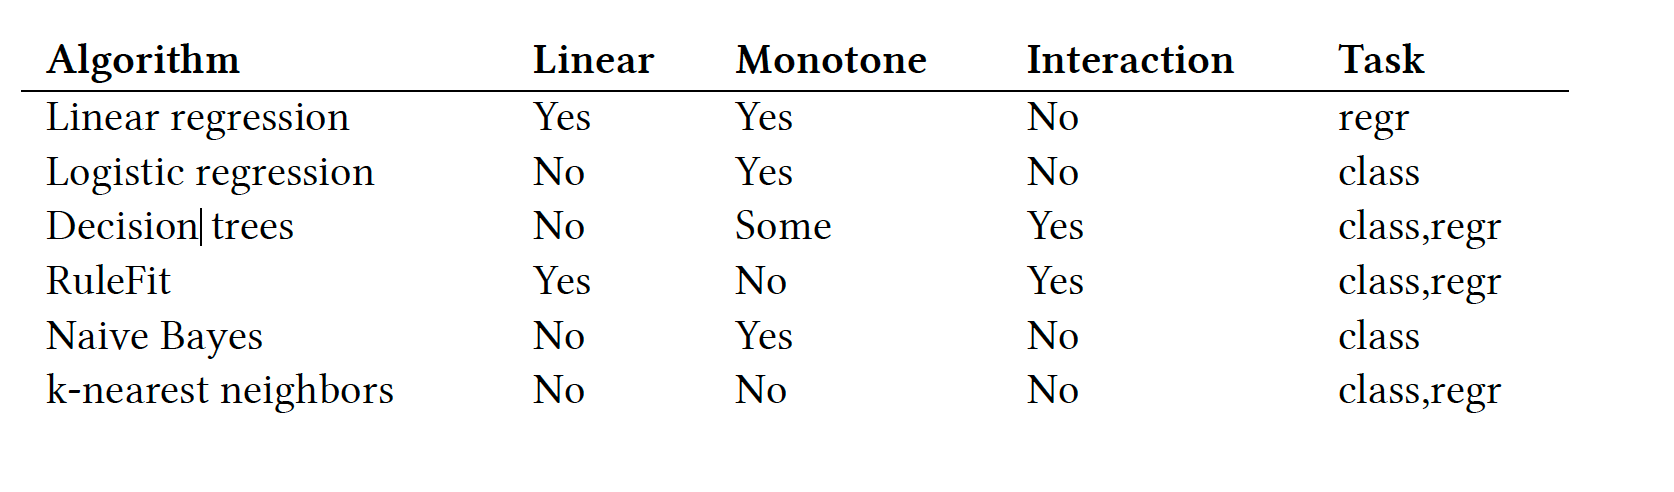
\includegraphics[width=0.7\textwidth]{img/int_models.png}
    \centering
\end{figure}
Some models allow to impose monotonicity and the possibility to include feature interactions.

\subsection{Linear Regression}
The dependent variable (target, prediction) is a weighted sum of the independent variables (predictors).
Linear models can be used to model the dependence of a regression target y on some features x. The learned relationships are linear and can be written for a single instance as follows:
\begin{equation}
    y=\beta_0+\beta_1x_1+\ldots+\beta_px_p+\epsilon
\end{equation}
The predicted outcome of an instance is a weighted sum of its $p$ features.
The betas ($\beta_j$) represent the learned feature weights or coefficients. 
The first weight in the sum ($\beta_0$) is called the intercept and is not multiplied with a feature.
The epsilon ($\epsilon$) is the error we still make, i.e. the difference between the prediction and the actual outcome. 
These errors are assumed to follow a Gaussian distribution, which means that we make errors in both negative and positive directions and make many small errors and few large errors.\\

Various methods can be used to estimate the optimal weight. The ordinary least squares method is usually used to find the weights that minimize the squared differences between the actual and the estimated outcomes:
\begin{equation}
    \hat{\boldsymbol{\beta}}=\arg\!\min_{\beta_0,\ldots,\beta_p}\sum_{i=1}^n\left(y^{(i)}-\left(\beta_0+\sum_{j=1}^p\beta_jx^{(i)}_{j}\right)\right)^{2}
\end{equation}

Estimated weights come with confidence intervals. A confidence interval is a range for the weight estimate that covers the “true” weight with a certain confidence. For example, a 95\% confidence interval for a weight of 
2 could range from 1 to 3. The interpretation of this interval would be: If we repeated the estimation 100 times with newly sampled data, the confidence interval would include the true weight in 95 out of 100 cases, given 
that the linear regression model is the correct model for the data.
\newif\ifgooditem
\gooditemtrue
\newcommand\gooditem{\gooditemtrue\item}
\newcommand\baditem{\gooditemfalse\item}

Whether the model is the “correct” model depends on whether the relationships in the data meet certain assumptions:
\begin{itemize}
    \item \textbf{Linearity}: The linear regression model forces the
    prediction to be a linear combination of features, which is both its
    greatest strength and its greatest limitation. Linearity leads to
    interpretable models. Linear effects are easy to quantify and describe. They
    are additive, so it is easy to separate the effects. If you suspect feature
    interactions or a nonlinear association of a feature with the target value,
    you can add interaction terms or use regression splines.
    \item \textbf{Normality}: It is assumed that the target outcome given the features follows a normal distribution. If this assumption is violated, the estimated confidence intervals of the feature weights are invalid.
    \item \textbf{Homoscedasticity} (constant variance): The variance of the error terms is assumed to be constant over the entire feature space.
    \item \textbf{Independence}: It is assumed that each instance is independent of any other instance. If you perform repeated measurements, such as multiple blood tests per patient, the data points are not independent.
    \item \textbf{Fixed features}: The input features are considered “fixed”. Fixed means that they are treated as “given constants” and not as statistical variables. This implies that they are free of measurement errors.
    \item \textbf{Absence of multicollinearity}: You do not want strongly correlated features, because this messes up the estimation of the weights. In a situation where two features are strongly correlated, it becomes problematic to estimate the weights because the feature effects are additive and it becomes indeterminable to which of the correlated features to attribute the effects.
\end{itemize}

\subsubsection{Interpretation}
The interpretation of a weight in the linear regression model depends on the type of the corresponding feature.
\begin{itemize}
    \item \textbf{Numerical feature}: Increasing the numerical feature by one unit changes the estimated outcome by its weight.
    \item \textbf{Binary feature}: A feature that takes one of two possible values for each instance. Changing the feature from the reference category to the other category changes the estimated outcome by the feature's weight.
    \item \textbf{Intercept $\beta_0$}Changing the feature from the reference category to the other category changes the estimated outcome by the feature's weight.
    The interpretation of the intercept is usually not relevant because instances with all features values at zero often make no sense. The interpretation is only meaningful when the features have been standardised (mean of zero, standard deviation of one). Then the intercept reflects the predicted outcome of an instance where all features are at their mean value.
\end{itemize}

\subsubsection{Explained Variance}
Another important measurement for interpreting linear models is the R-squared measurement.
R-squared tells you how much of the total variance of your target outcome is explained by the model. The higher R-squared, the better your model explains the data. 
The formula for calculating R-squared is:
\begin{equation*}
    R^2=1-SSE/SST
\end{equation*}
SSE is the squared sum of the error terms:
\begin{equation*}
    SSE=\sum_{i=1}^n(y^{(i)}-\hat{y}^{(i)})^2
\end{equation*}
SST is the squared sum of the data variance:
\begin{equation*}
    SST=\sum_{i=1}^n(y^{(i)}-\bar{y})^2
\end{equation*}
The SSE tells you how much variance remains after fitting the linear model, which is measured by the squared differences between the predicted and actual target values.
SST is the total variance of the target outcome. R-squared tells you how much of your variance can be explained by the linear model. R-squared usually ranges between 0 
for models where the model does not explain the data at all and 1 for models that explain all of the variance in your data.\\

It is also possible for R-squared to take on a negative value without violating any mathematical rules.
This happens when SSE is greater than SST which means that a model does not capture the trend of the data and fits to the data worse than using the mean of the target as the prediction.\\

There is a catch, because R-squared increases with the number of features in the model, even if they do not contain any information about the target value at all. 
Therefore, it is better to use the adjusted R-squared, which accounts for the number of features used in the model. 
Its calculation is:
\begin{equation*}
    \bar{R}^2=1-(1-R^2)\frac{n-1}{n-p-1}
\end{equation*}
where p is the number of features and n the number of instances.

It is not meaningful to interpret a model with very low (adjusted) R-squared, because such a model basically does not explain much of the variance. Any interpretation of the weights would not be meaningful.

\subsubsection{Feature Importance}
The importance of a feature in a linear regression model can be measured by the absolute value of its t-statistic. 
The t-statistic is the estimated weight scaled with its standard error.
\begin{equation*}
    t_{\hat{\beta}_j}=\frac{\hat{\beta}_j}{SE(\hat{\beta}_j)}
\end{equation*}
Let us examine what this formula tells us: The importance of a feature increases with increasing weight. This makes sense.
The more variance the estimated weight has (= the less certain we are about the correct value), the less important the feature is. 
This also makes sense.
\subsubsection{Visual Interpretation}
Various visualizations make the linear regression model easy and quick to grasp for humans.\\

\textbf{Weight Plot}
The information of the weight table (weight and variance estimates) can be visualized in a weight plot. The following plot shows the results from the previous linear regression model.
\begin{figure}[H]
    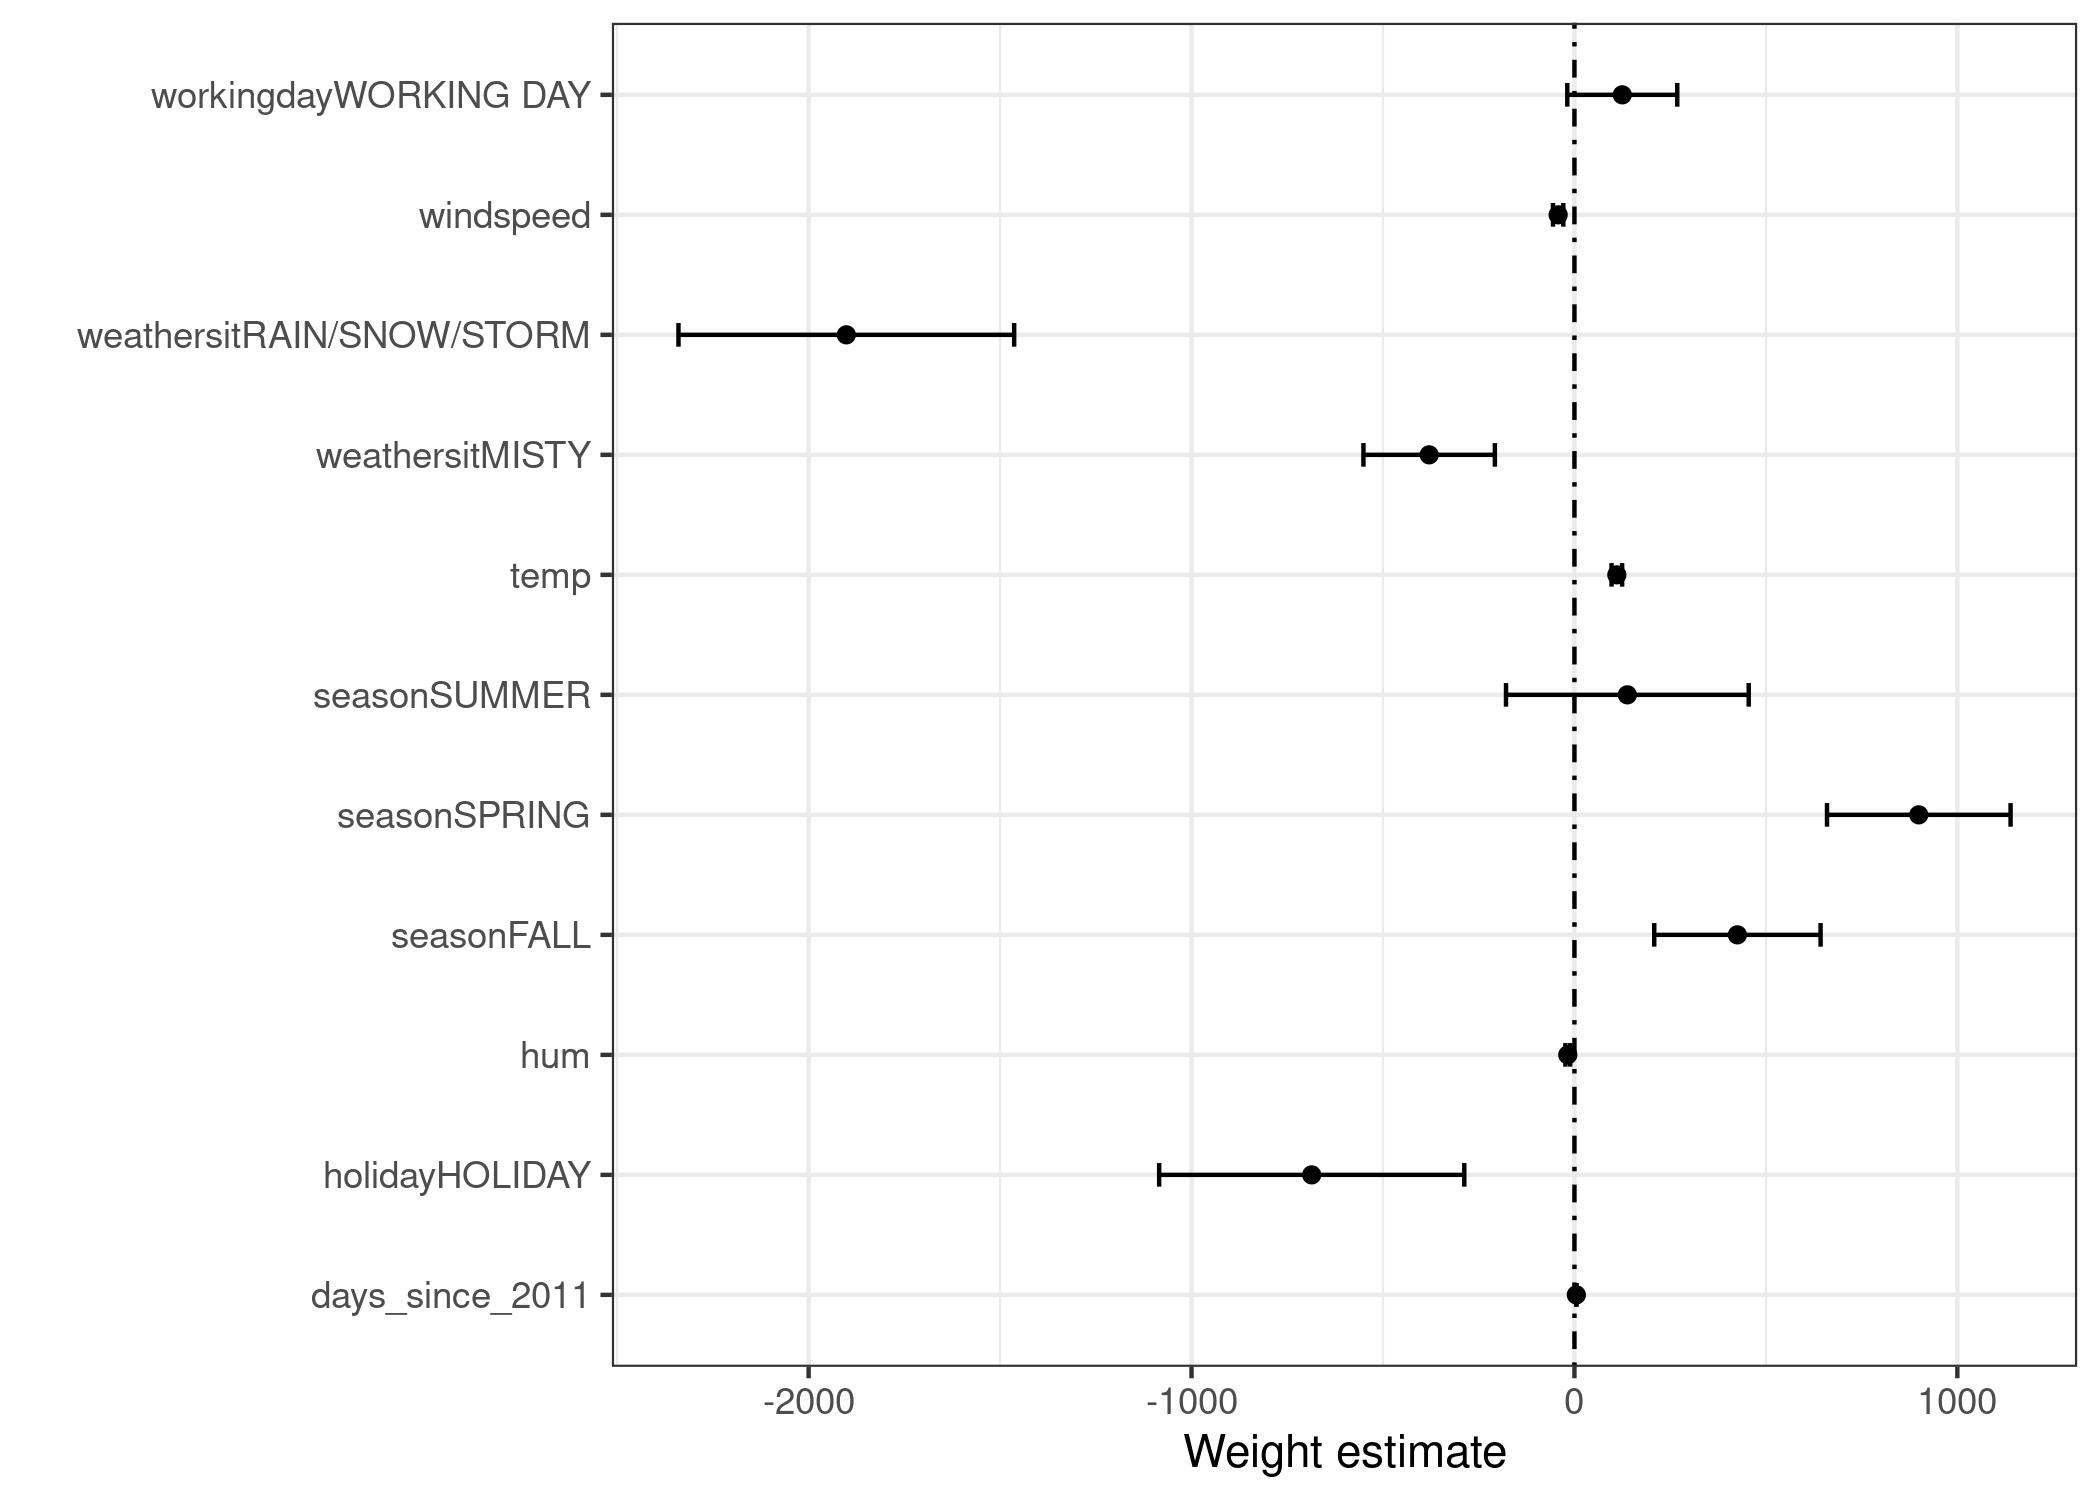
\includegraphics[width=0.5\textwidth]{img/linear-weights-plot-1.jpeg}
    \centering
\end{figure}

The problem with the weight plot is that the features are measured on different scales.
You can make the estimated weights more comparable by scaling the features (zero mean and standard deviation of
one) before fitting the linear model.\\

\textbf{Effect plot}
The weights of the linear regression model can be more meaningfully analyzed when they are multiplied by the actual feature values.
It is also important to know the distribution of your feature in the data, because if you have a very low variance, it means that almost 
all instances have similar contribution from this feature. 
The effect plot can help you understand how much the combination of weight and feature contributes to the predictions in your data. Start by calculating the effects, 
which is the weight per feature times the feature value of an instance:
\begin{equation*}
    \text{effect}_{j}^{(i)}=w_{j}x_{j}^{(i)}
\end{equation*}
The effects can be visualized with boxplots. The box in a boxplot contains the effect range for half of the data (25\% to 75\% effect quantiles). 
The vertical line in the box is the median effect, i.e. 50\% of the instances have a lower and the other half a higher effect on the prediction. The dots are outliers, defined as points that are more than 1.5 * IQR (interquartile range, that is, the difference between the first and third quartiles) above the third quartile, or less than 1.5 * IQR below the first quartile. 
The two horizontal lines, called the lower and upper whiskers, connect the points below the first quartile and above the third quartile that are not outliers. If there are no outliers the whiskers will extend to the minimum and maximum values.
\begin{figure}[H]
    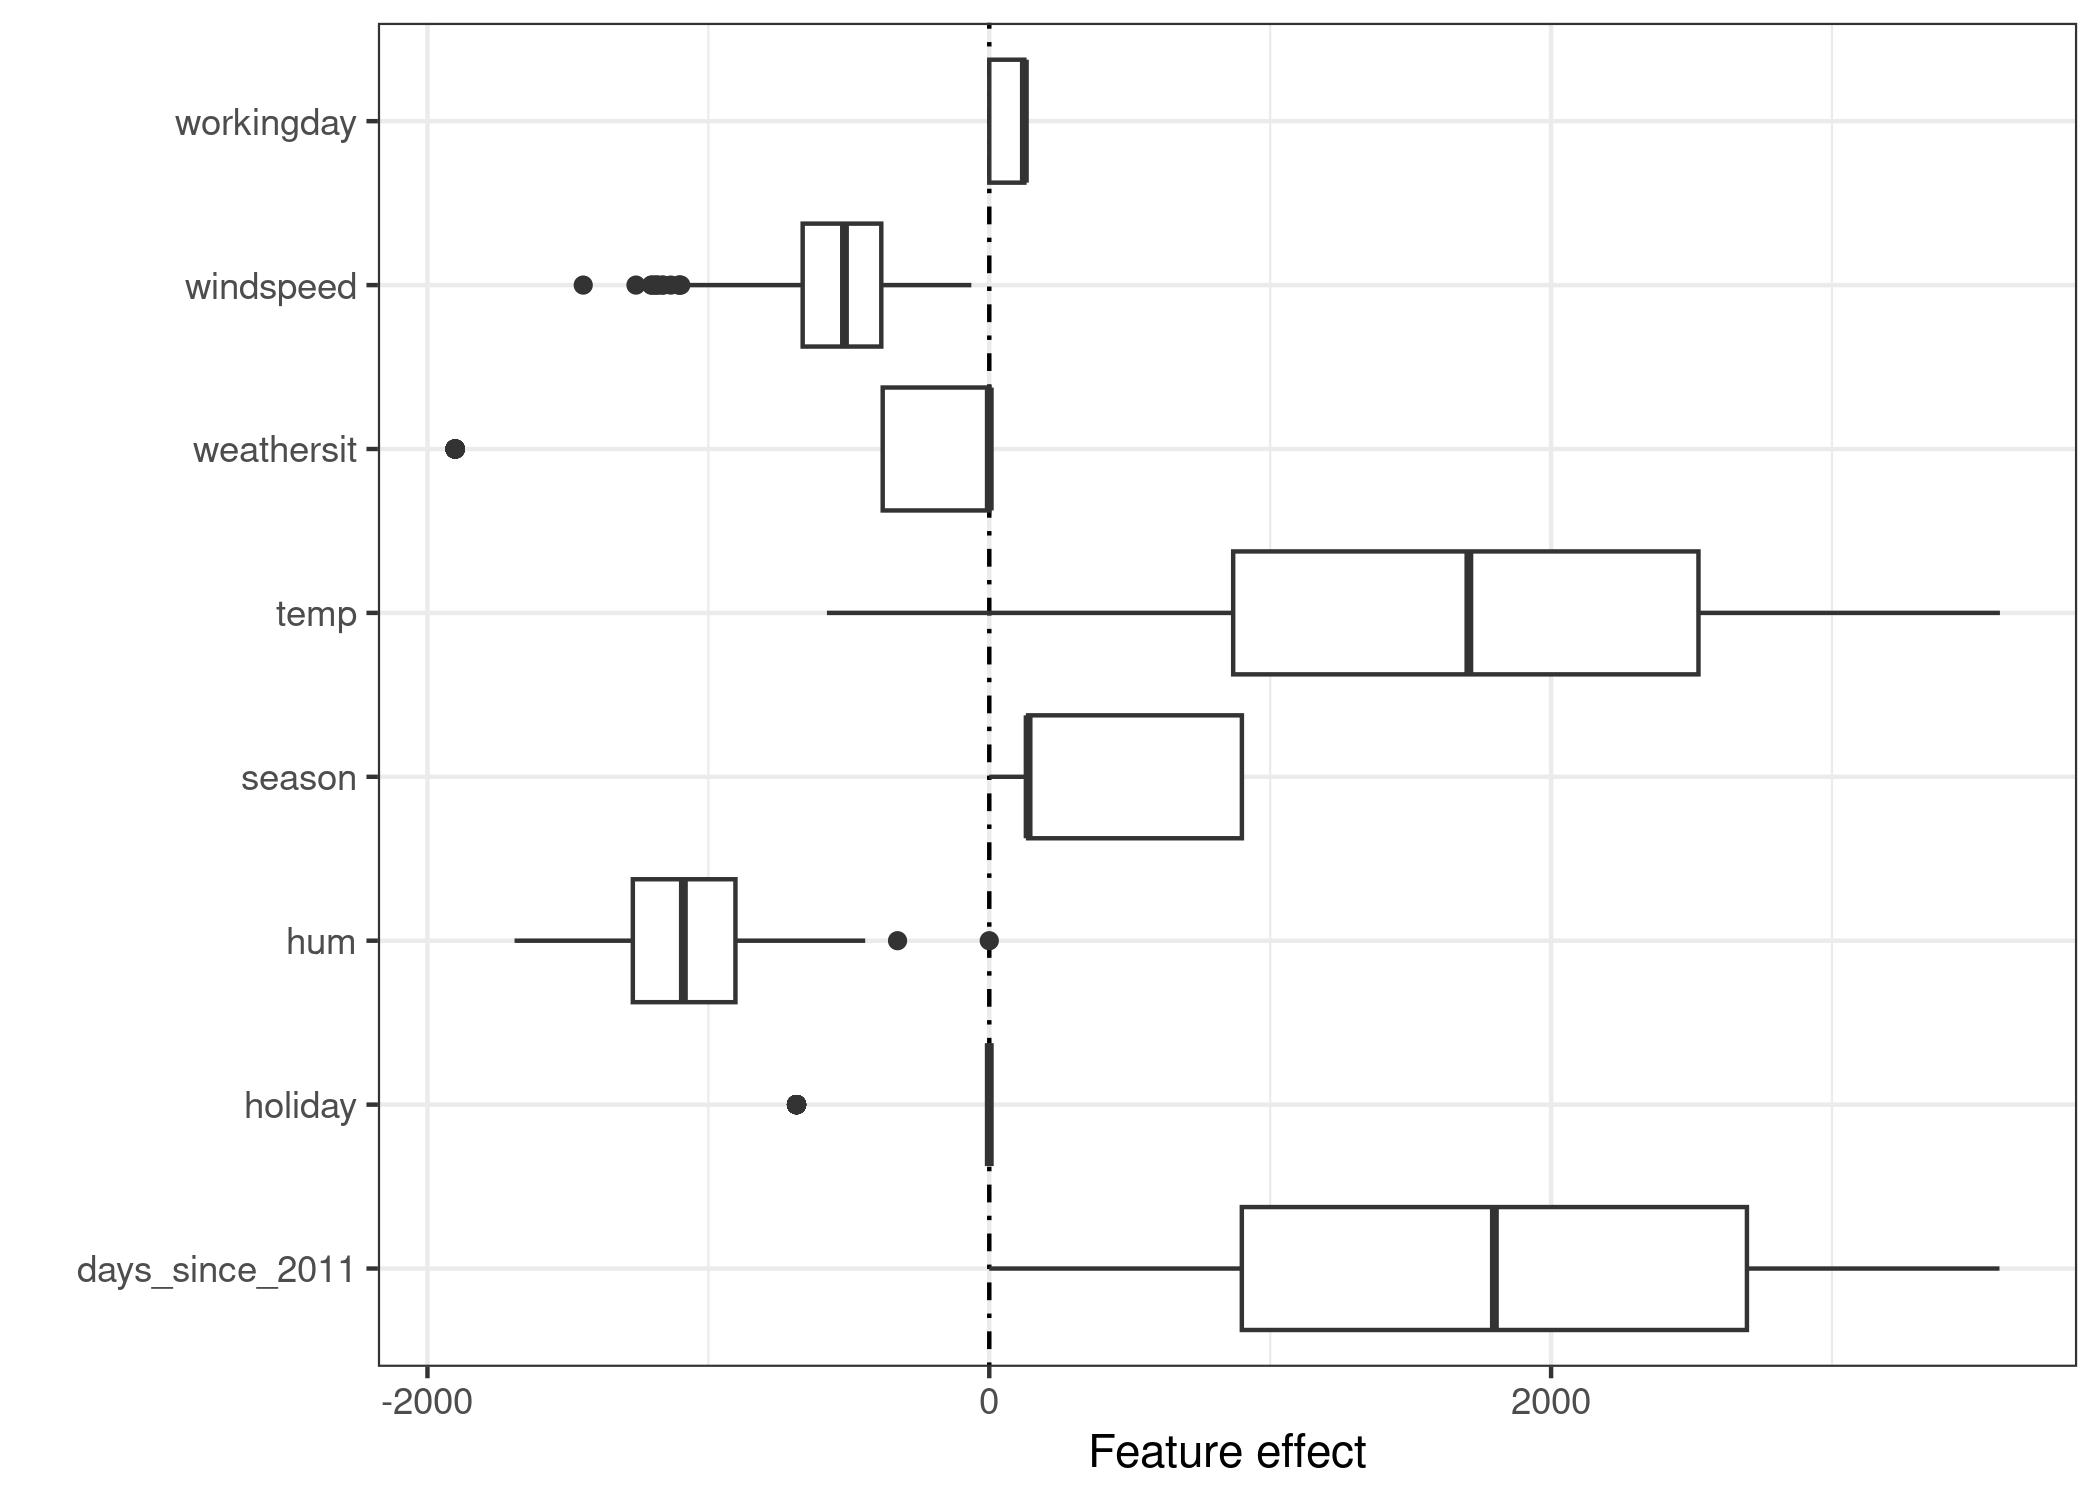
\includegraphics[width=0.5\textwidth]{img/linear-effects-1.jpeg}
    \centering
\end{figure}

\subsubsection{Explain Individual Predictions}
How much has each feature of an instance contributed to the prediction? 
This can be answered by computing the effects for this instance. That is multiplying the feature values for this instance times the corresponding weights.
We add these individual effects as crosses to the effect plot, which shows us the distribution of the effects in the data. This allows us to compare the individual effects with the distribution
of effects in the data.
\begin{figure}[H]
    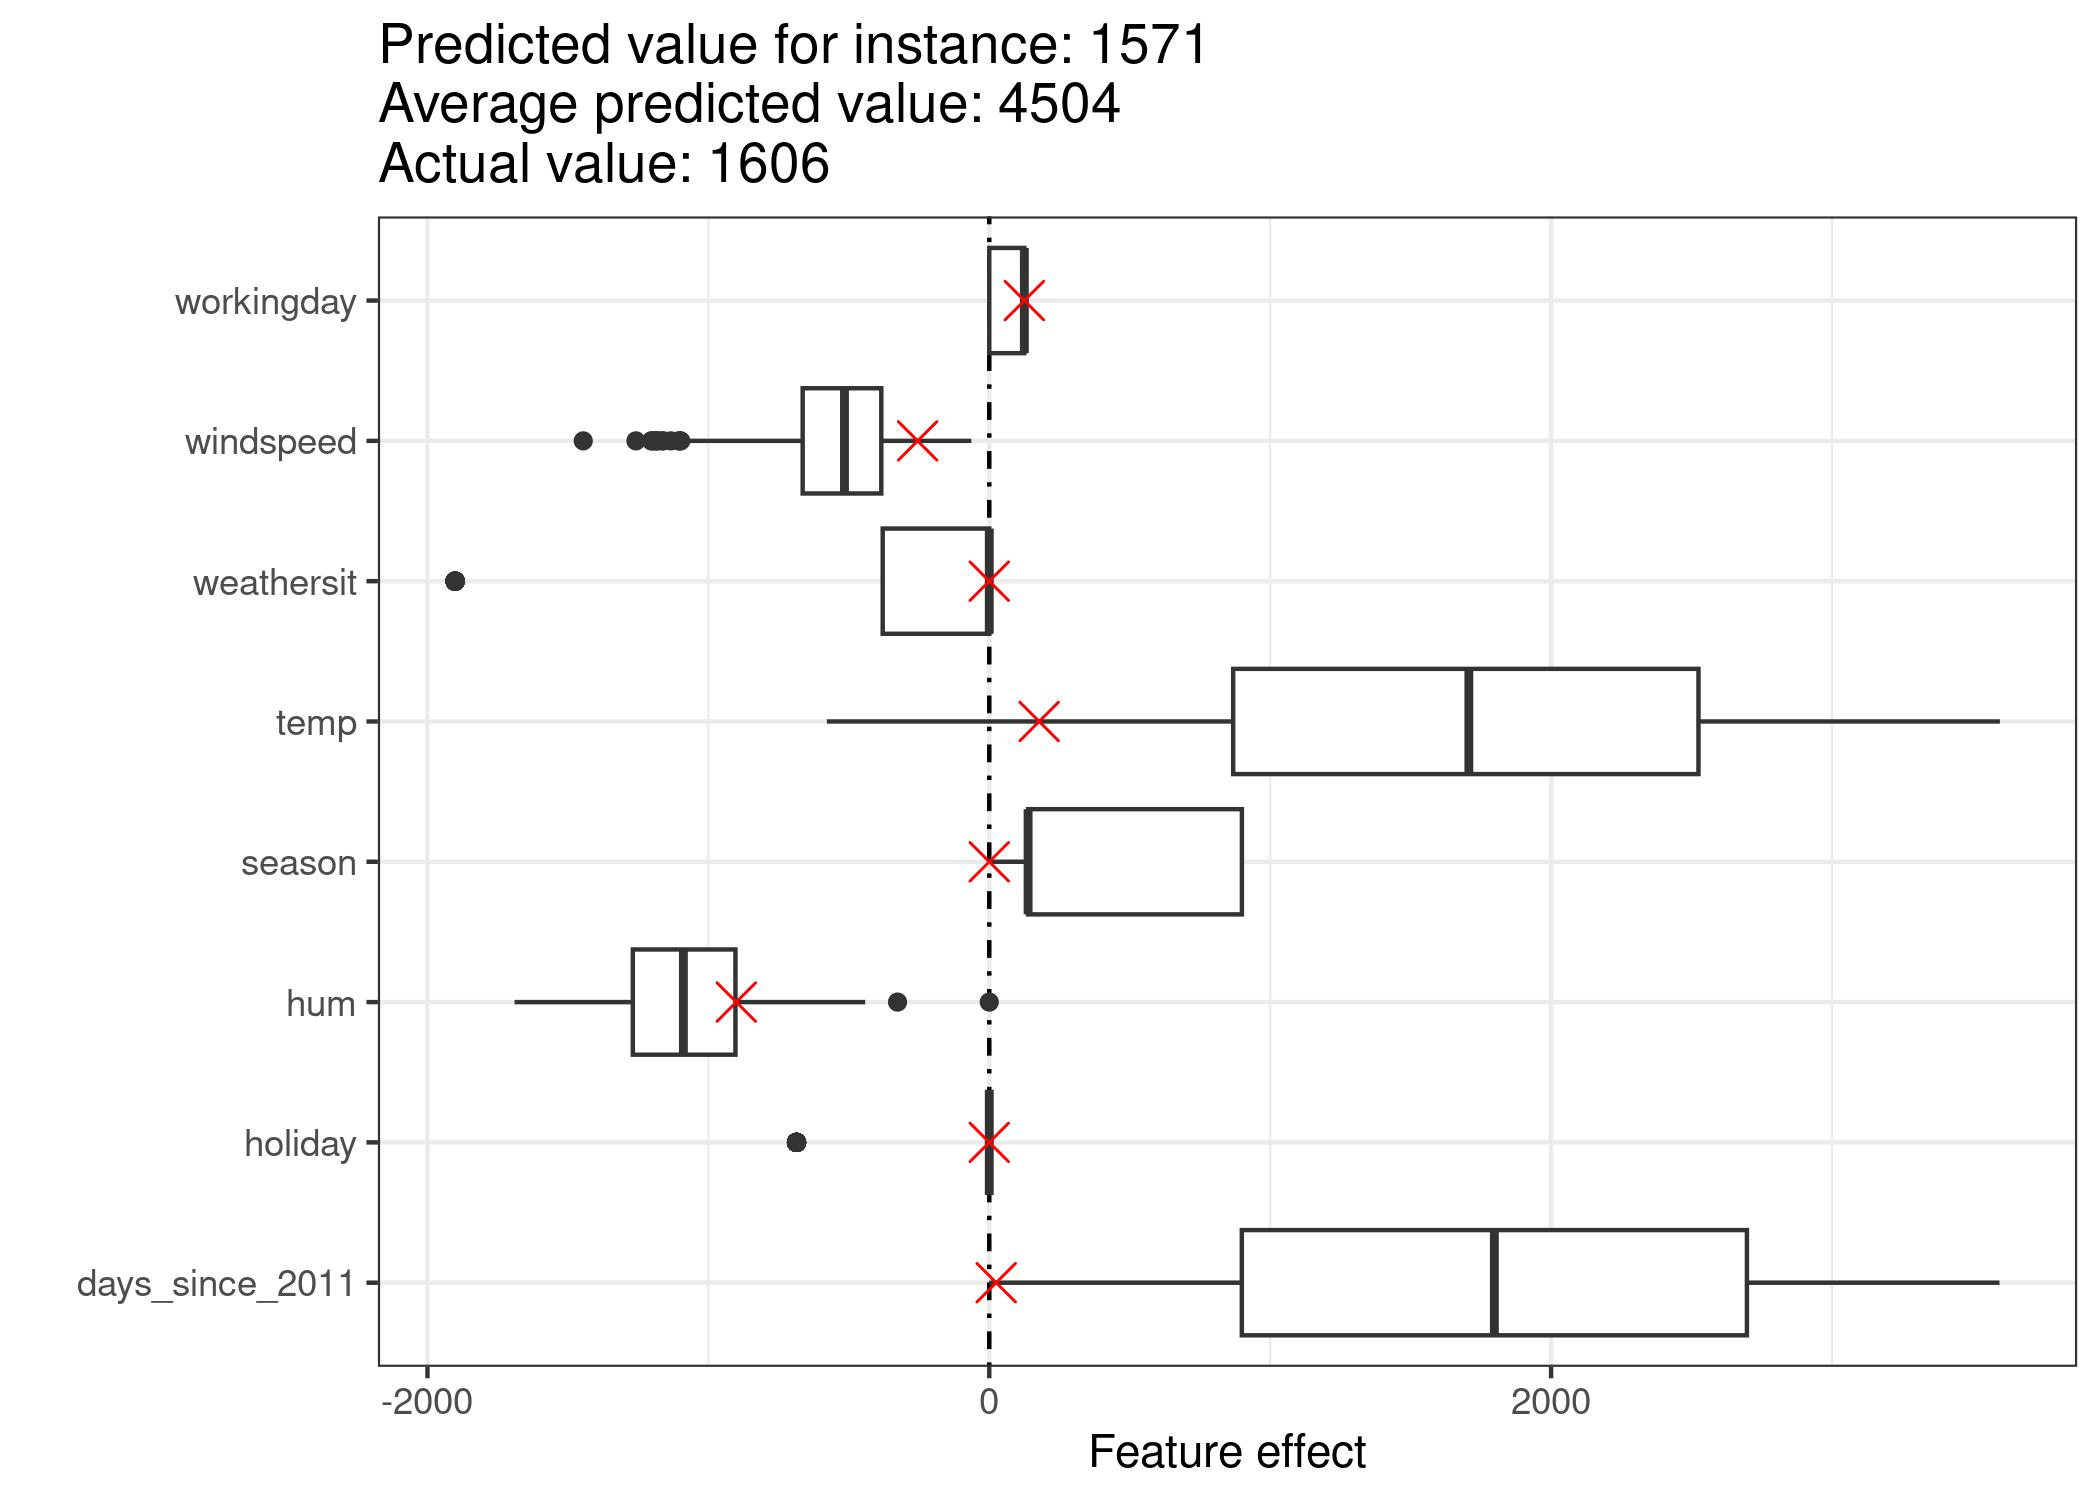
\includegraphics[width=0.5\textwidth]{img/linear-effects-single-1.jpeg}
    \centering
\end{figure}
\subsubsection{Do Linear Models Create Good Explanations?}
Judging by the attributes that constitute a good explanation, as presented previously, linear models do not create the best explanations. 
% https://tex.stackexchange.com/a/101296
\begin{itemize}[label={\ifgooditem\color{green}\else\color{red}\fi\textbullet}]
\gooditem Contrastive (allows to compare the contributions of different features)
\gooditem Simple
\gooditem Generate truthful explanations if it fits well the data
\baditem Applicable only when linear relations hold
\baditem Do not directly account for feature interactions
\baditem Not suitable for multicollinear features
\baditem Standard error increases with the number of features
\end{itemize}

\subsubsection{Lasso Regression}
Lasso stands for "least absolute shrinkage and selection operator" this tecnique is an automatic and convenient way to introduce sparsity (i.e use few features) into the linear regression model.
When applied in a linear regression model, performs feature selection and regularization of the selected feature weights.
Let us consider the minimization problem that the weights optimize:
\begin{equation*}
    min_{\boldsymbol{\beta}}\left(\frac{1}{n}\sum_{i=1}^n(y^{(i)}-x_i^T\boldsymbol{\beta})^2\right)
\end{equation*}
Lasso adds a term to this optimization problem.
\begin{equation*}
    min_{\boldsymbol{\beta}}\left(\frac{1}{n}\sum_{i=1}^n(y^{(i)}-x_{i}^T\boldsymbol{\beta})^2+\lambda||\boldsymbol{\beta}||_1\right)
\end{equation*}
The term $||\boldsymbol{\beta}||_1$, the L1-norm of the feature vector, leads to a penalization of large weights. 
Since the L1-norm is used, many of the weights receive an estimate of 0 and the others are shrunk.
The parameter lambda ($\lambda$) controls the strength of the regularizing effect and is usually tuned by cross-validation. 
Especially when lambda is large, many weights become 0.

\subsubsection{Other methods for sparsity in linear models}
A wide spectrum of methods can be used to reduce the number of features in a linear model.

Pre-processing methods:
\begin{itemize}
    \item \textbf{Manually selected features}: You can always use expert knowledge to select or discard some features. The big drawback is that it cannot be automated and you need to have access to someone who understands the data
    \item \textbf{Univariate selection}: An example is the correlation coefficient. You only consider features that exceed a certain threshold of correlation between the feature and the target. The disadvantage is that it only considers the features individually. Some features might not show a correlation until the linear model has accounted for some other features. Those ones you will miss with univariate selection methods.
\end{itemize}

Step-wise methods:
\begin{itemize}
    \item \textbf{Forward selection}: Fit the linear model with one feature. Do this with each feature. Select the model that works best (e.g. highest R-squared). Now again, for the remaining features, fit different versions of your model by adding each feature to your current best model. Select the one that performs best. Continue until some criterion is reached, such as the maximum number of features in the model.
    \item \textbf{Backward selection}: Similar to forward selection. But instead of adding features, start with the model that contains all features and try out which feature you have to remove to get the highest performance increase. Repeat this until some stopping criterion is reached.
\end{itemize}

\subsubsection{Main issues of linear models and how to overcome them}
\begin{figure}[H]
    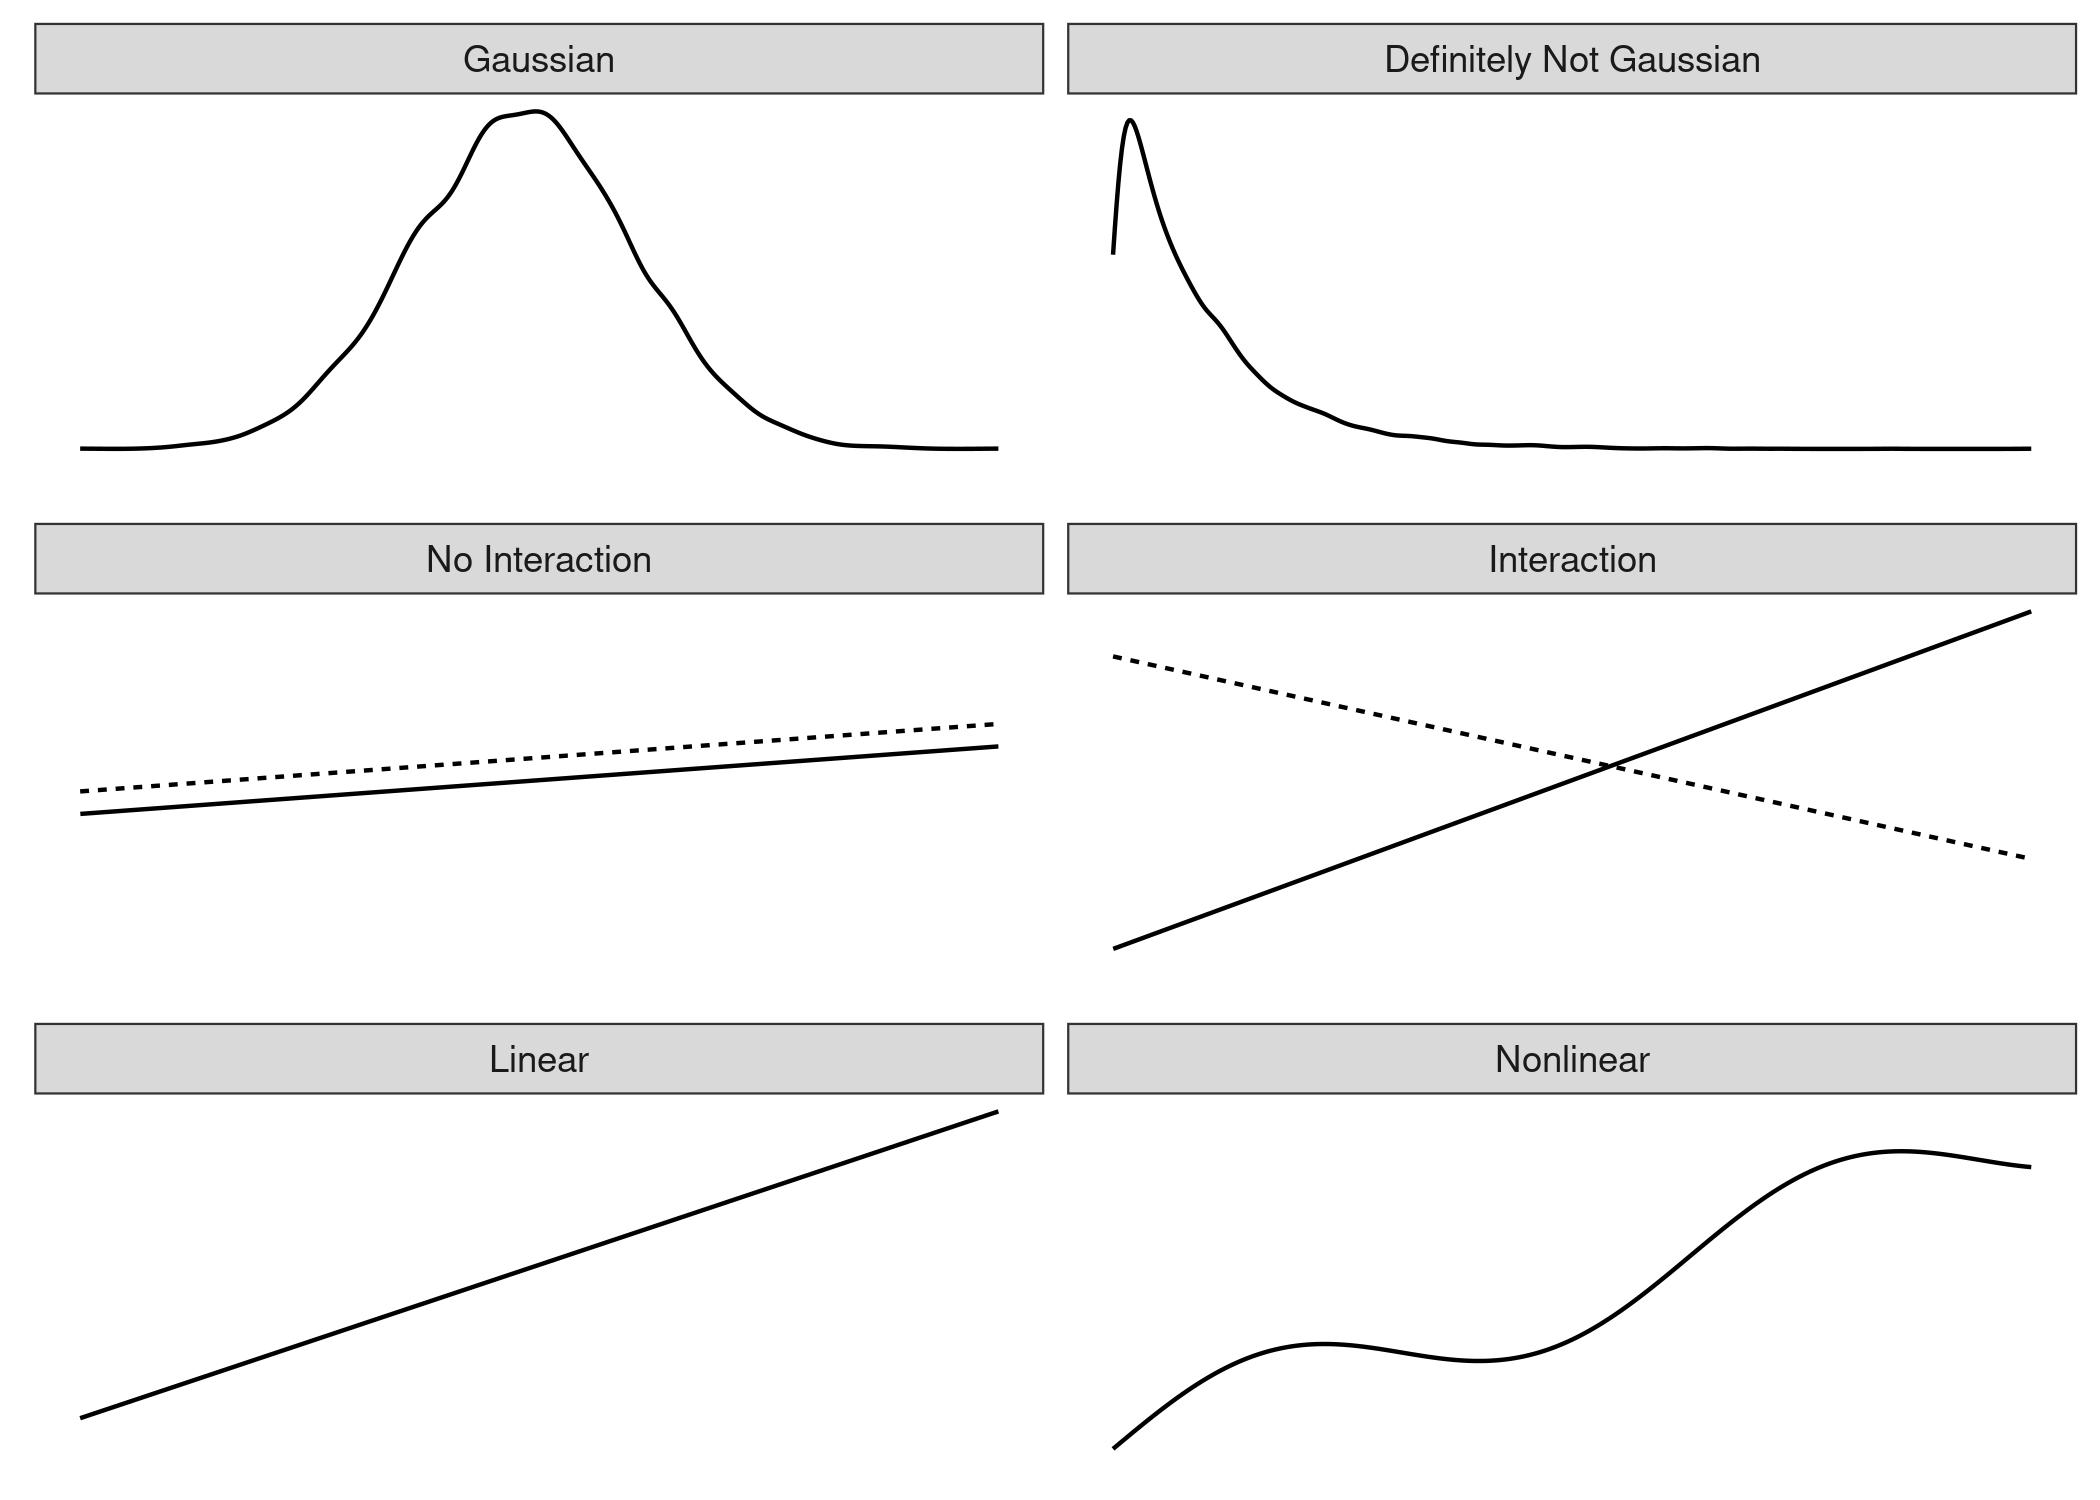
\includegraphics[width=0.5\textwidth]{img/three-lm-problems-1.jpeg}
    \centering
    \caption{Three assumptions of the linear model (left side): Gaussian distribution of the outcome given the features, additivity (= no interactions) and linear relationship. Reality usually does not adhere to those assumptions (right side): Outcomes might have non-Gaussian distributions, features might interact and the relationship might be nonlinear.}
\end{figure}
The biggest strength but also the biggest weakness of the linear regression model is that the prediction is modeled as a weighted sum of the features. In addition, the linear model comes with many other assumptions. The bad news is (well, not really news) that all those assumptions are often violated in reality: The outcome given the features might have a non-Gaussian distribution, the features might interact and the relationship between the features and the outcome might be nonlinear. The good news is that the statistics community has developed a variety of modifications that transform the linear regression model from a simple blade into a Swiss knife.

There is a solution to all these problems:
\begin{enumerate}
    \item \textbf{the target outcome y given the features does not follow a Gaussian distribution.} 
    Suppose I want to predict how many minutes I will ride my bike on a given day. As features I have the type of day, the weather and so on. If I use a linear model, it could predict negative minutes because it assumes a Gaussian distribution which does not stop at 0 minutes. Also if I want to predict probabilities with a linear model, I can get probabilities that are negative or greater than 1. 
    The solution to this is to use Generalized Linear Models (GLMs for short), which are an extention to Linear Regression, that wraps the weighted sum of the features into a non-linear function and allows non-gaussian errors.
    \item \textbf{The features interact}: To predict the number of bicycles rented, there may be an interaction between temperature and whether it is a working day or not. Perhaps, when people have to work, the temperature does not influence the number of rented bikes much, because people will ride the rented bike to work no matter what happens. On days off, many people ride for pleasure, but only when it is warm enough. When it comes to rental bicycles, you might expect an interaction between temperature and working day.
    The solution to this id to add a column to the feature matrix that represens the interaction between the features and fit the model as usual.
    \item \textbf{The true relationship between the features and y is not linear}:  Linearity in linear models means that no matter what value an instance has in a particular feature. For example the relation between the temperature and the number of rental bikes, if there are 10 degrees outside and the temperature increases by one degree the change in the number of rental bikes is not same as if outside there 40 degrees and the temperature increases by one degree.
    Intuitively, one expects that increasing the temperature from 10 to 11 degrees Celsius has a positive effect on bicycle rentals and from 40 to 41 a negative effect. There are various solutions to this problem: 
    \begin{itemize}
        \item Feature transformation: apply a transformation (e.g logarithm) to the feature
        \item Feature categorization: Another possibility to achieve a nonlinear effect is to discretize the feature; turn it into a categorical feature. For example, you could cut the temperature feature into 20 intervals with the levels [-10, -5), [-5, 0), … and so on.
        \item Generalized Additive Models (GAMs): Why not 'simply' allow the (generalized) linear model to learn nonlinear relationships?That is the motivation behind GAMs. GAMs relax the restriction that the relationship must be a simple weighted sum, and instead assume that the outcome can be modeled by a sum of arbitrary functions of each feature. Mathematically, the relationship in a GAM looks like this: $g(E_Y(y|x))=\beta_0+f_1(x_{1})+f_2(x_{2})+\ldots+f_p(x_{p})$
    \end{itemize}
\end{enumerate}

\begin{figure}[H]
    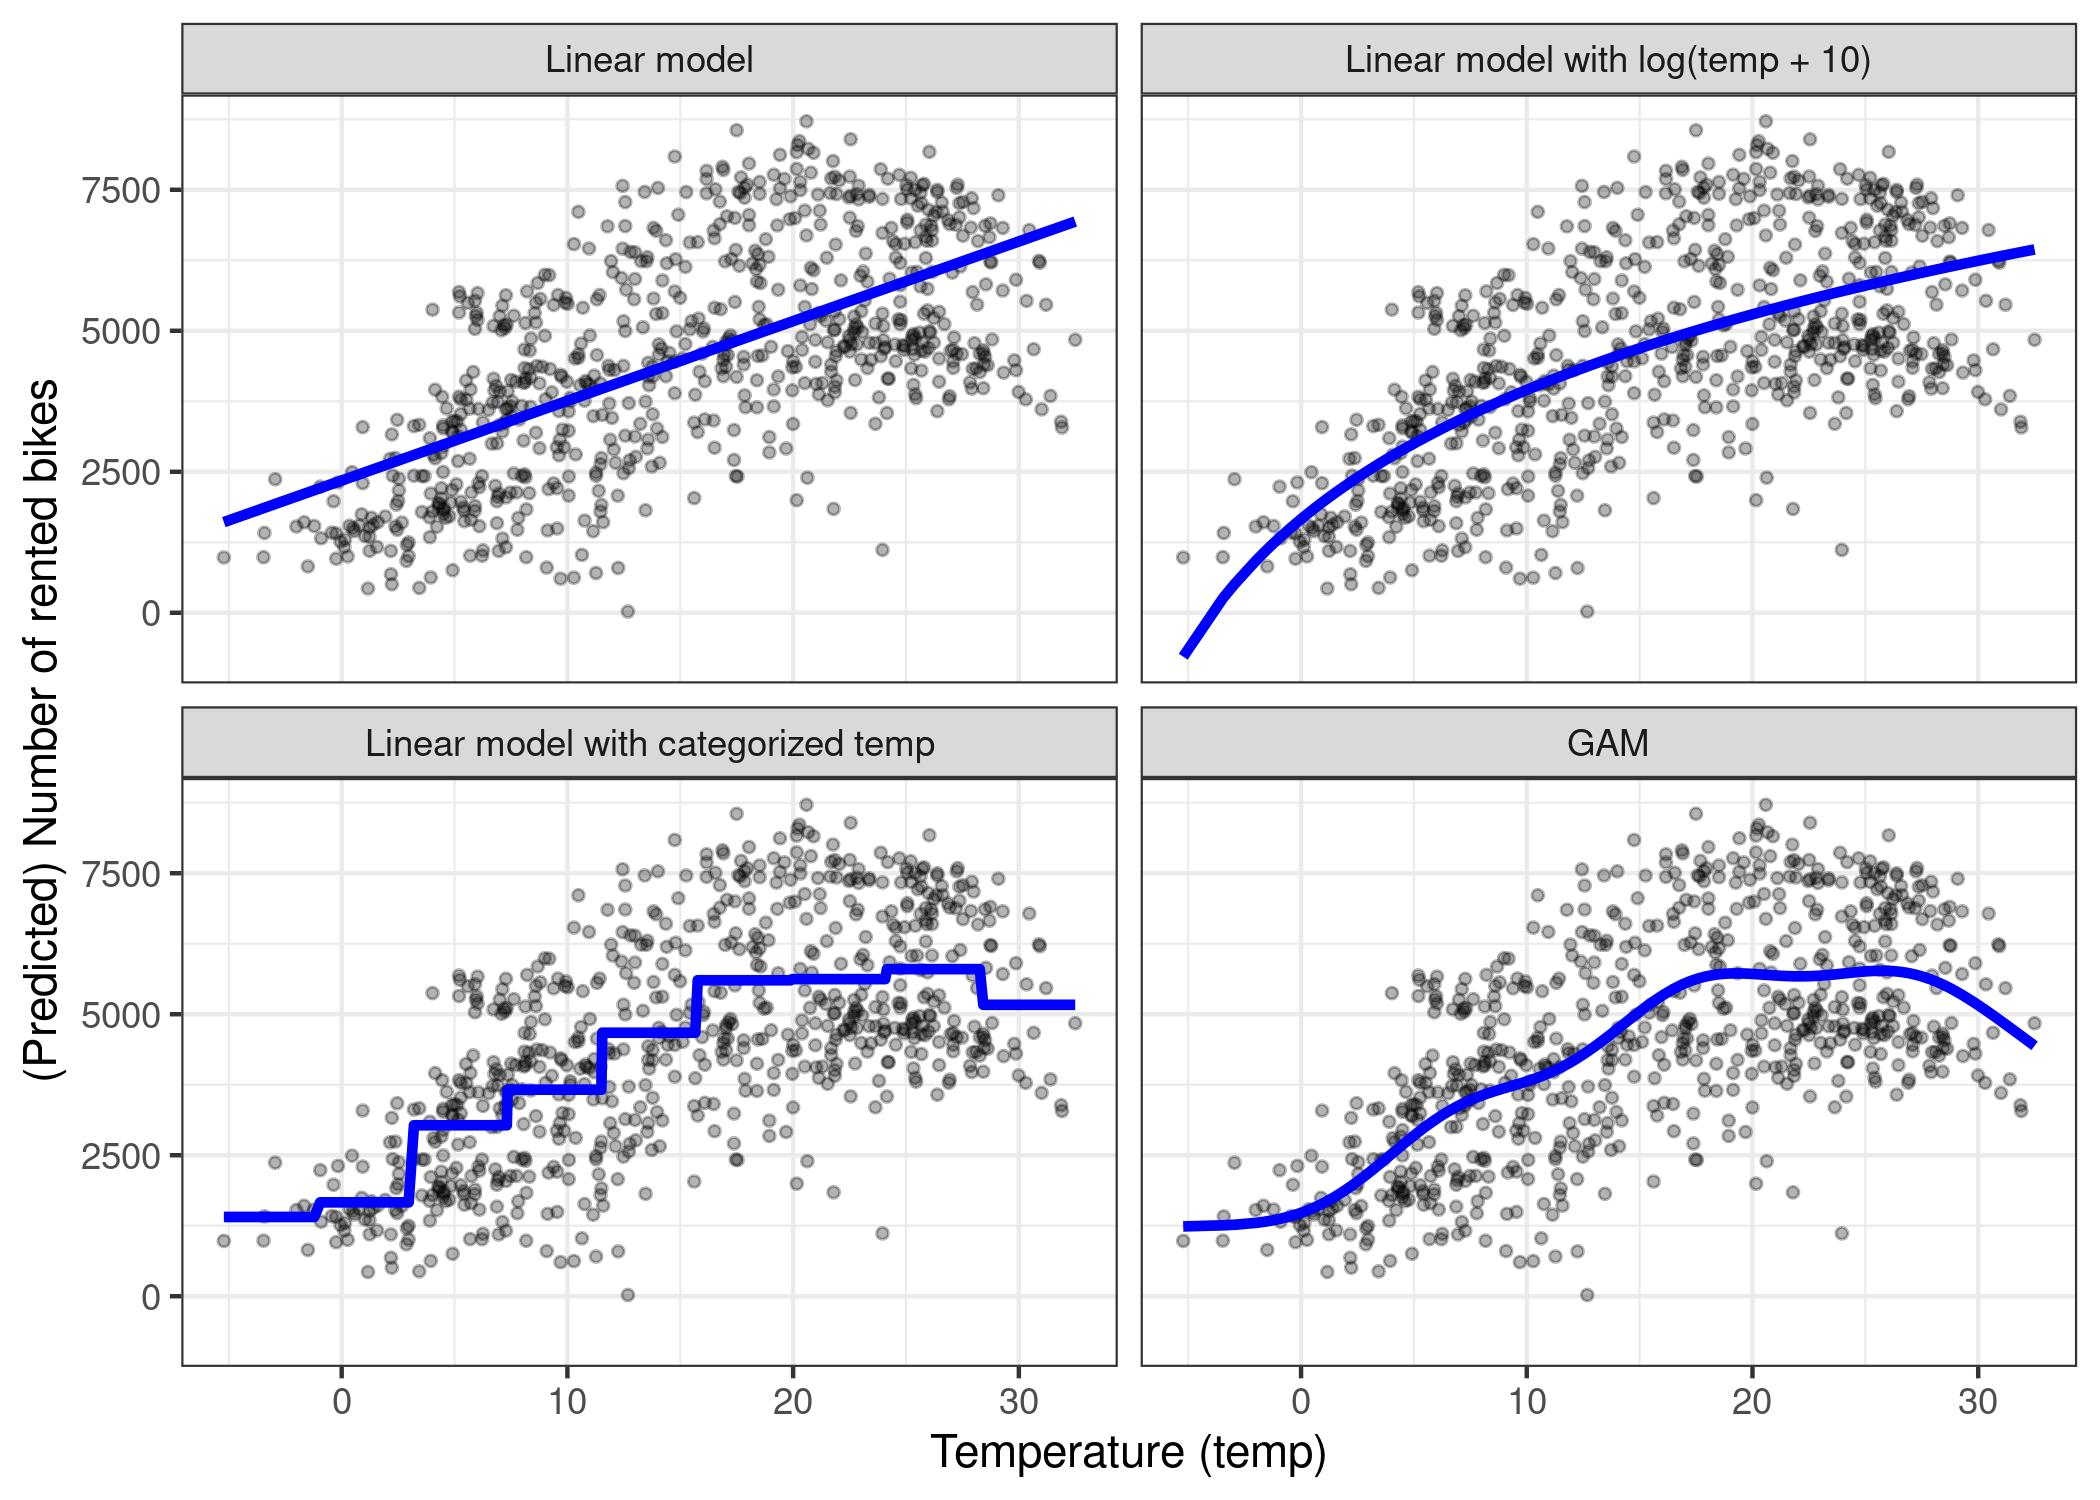
\includegraphics[width=0.7\textwidth]{img/nonlinear-effects-1.jpeg}
    \centering
    \caption{Predicting the number of rented bicycles using only the temperature feature. A linear model (top left) does not fit the data well. One solution is to transform the feature with e.g. the logarithm (top right), categorize it (bottom left), which is usually a bad decision, or use Generalized Additive Models that can automatically fit a smooth curve for temperature (bottom right).}
\end{figure}

Most modifications of the linear model make the model less interpretable.

\subsection{Decision Trees}
Linear regression and logistic regression models fail in situations where the relationship
between features and outcome is nonlinear or where features interact with each other.\\

Tree based models split the data multiple times according to certain cutoff values in the features. Through splitting, different subsets of the dataset are created, with each instance belonging to one subset. The final subsets are called terminal or leaf nodes and the intermediate subsets are called internal nodes or split nodes. To predict the outcome in each leaf node, the average outcome of the training data in this node is used. Trees can be used for classification and regression.\\

There are various algorithms that can grow a tree. They differ in the possible structure of the tree (e.g. number of splits per node), the criteria how to find the splits, when to stop splitting and how to estimate the simple models within the leaf nodes. The classification and regression trees (CART) algorithm is probably the most popular algorithm for tree induction.
The following formula describes the relationship between the outcome y and features x.
\begin{equation*}
    \hat{y}=\hat{f}(x)=\sum_{m=1}^Mc_m{}I\{x\in{}R_m\}
\end{equation*}
Each instance falls into exactly one leaf node (=subset $R_m$). $I_{\{x\in{}R_m\}}$ is the identity function that returns 1 if $x$ is in the subset $R_m$ and 0 otherwise. If an instance falls into a leaf node $R_l$, the predicted outcome is $\hat{y}=c_l$, where $c_l$ is the average of all training instances in leaf node $R_l$.

\subsubsection{Splitting criterion}
The best cut-off point makes the two resulting subsets as different as possible with respect to the target outcome.\\
CART takes a feature and determines which cut-off point minimizes the variance of y for a regression task or the Gini index of the class distribution of y for classification tasks. The variance tells us how much the y values in a node are spread around their mean value. The Gini index tells us how “impure” a node is, e.g. if all classes have the same frequency, the node is impure, if only one class is present, it is maximally pure.\\

The algorithm continues this search-and-split recursively in both new nodes until a stop
criterion is reached. Possible criteria are:
\begin{itemize}
    \item A minimum number of instances that have to be in a node before the split
    \item The minimum number of instances that have to be in a terminal node.
\end{itemize}

\subsubsection{Interpretation}
\begin{itemize}
    \item \textbf{Straightforward:} starting from the root node, you go to the next nodes and the edges tell you
    which subsets you are looking at until you reach the terminal node.
    \item \textbf{Feature importance:} Go through all the splits for which the feature was used and measure how much it has reduced the
    variance or Gini index compared to the parent node. The sum of all importances is scaled to 100. This means that each importance can be interpreted as share of the overall model importance.
    \item \textbf{Tree decomposition:} Individual predictions of a decision tree can be explained by decomposing the decision path into one component per feature. We can track a decision through the tree and explain a prediction by the contributions added at each decision node.
    The root node in a decision tree is our starting point. If we were to use the root node to make predictions, it would predict the mean of the outcome of the training data. With the next split, we either subtract or add a term to this sum, depending on the next node in the path. To get to the final prediction, we have to follow the path of the data instance that we want to explain and keep adding to the formula.
    \begin{equation*}
        \hat{f}(x)=\bar{y}+\sum_{d=1}^D\text{split.contrib(d,x)}=\bar{y}+\sum_{j=1}^p\text{feat.contrib(j,x)}
    \end{equation*}
    The prediction of an individual instance is the mean of the target outcome plus the sum of all contributions of the D splits that occur between the root node and the terminal node where the instance ends up. We are not interested in the split contributions though, but in the feature contributions. A feature might be used for more than one split or not at all. We can add the contributions for each of the p features and get an interpretation of how much each feature has contributed to a prediction.
\end{itemize}


